\documentclass{article}
\usepackage{amsmath, amssymb, amsfonts}
\usepackage[utf8]{inputenc}
\usepackage[english]{babel}
\usepackage{fontenc}
\usepackage{graphicx}
\usepackage{geometry}
\usepackage{fancyhdr}
\usepackage{titlesec}
\usepackage{microtype}
\usepackage{float}
\usepackage{hyperref}
\usepackage{cleveref}
\usepackage{placeins}
\usepackage{subcaption}
\usepackage{mdframed}

\geometry{a4paper, margin=1in}
\setlength{\headheight}{32.05278pt}

\pagestyle{fancy}
\fancyhf{}
\fancyhead[L]{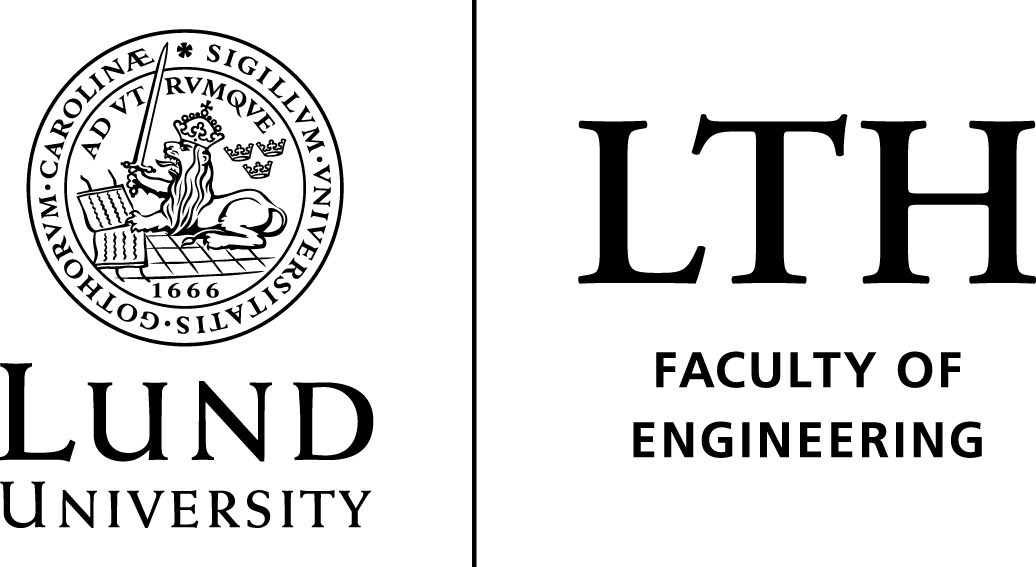
\includegraphics[height=1cm]{lth.png}}
\fancyhead[C]{Sim Tools - Project 2}
\fancyhead[R]{Campoli, Cullen, Ghigliani \& Mutz}
\fancyfoot[L]{\today}
\fancyfoot[C]{\thepage}
\fancyfoot[R]{Exchange Students}

\titleformat{\section}
  {\Large\bfseries\sffamily}
  {\thesection.}{0.5em}{}
\titlespacing*{\section}{0pt}{1.5ex plus 1ex minus .2ex}{1ex plus .2ex}

\begin{document}

\begin{titlepage}
    \centering
    \vspace*{1.5cm}
    {\LARGE\bfseries Simulation Tools\par}
    \vspace*{0.5cm}
    {\LARGE\bfseries Project 2\par}
    \vspace*{0.5cm}
    {\LARGE\bfseries Simulation of Differential-Algebraic Equations\par}
    \vspace{1cm}
    {\Large Campoli, Lucas\par}
    \vspace{0.5cm}
    {\Large Cullen de Erquiaga, Magdalena Itziar\par}
    \vspace{0.5cm}
    {\Large Ghigliani, Franco Agustín\par}
    \vspace{0.5cm}
    {\Large Mutz, Matias\par}
    \vspace{1cm}
    {\large Exchange Students\par}
    \vspace{2cm}
    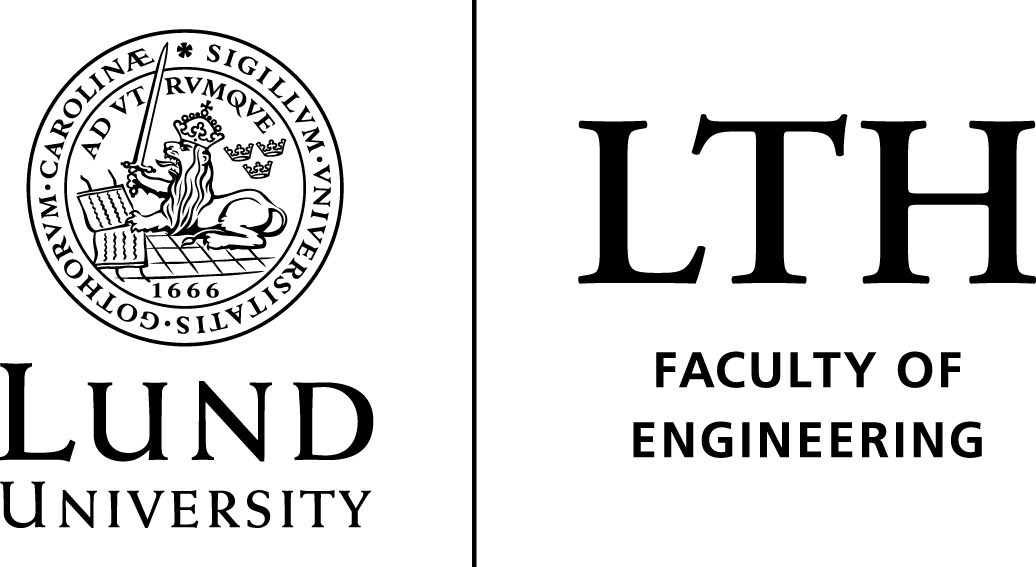
\includegraphics[width=0.7\textwidth]{lth.png}
    \vfill
    {\large \today\par}
\end{titlepage}

\tableofcontents
\newpage

\phantomsection
\section*{Introduction}
\addcontentsline{toc}{section}{Introduction}
\indent

This report presents Part II of the course project, focusing on the implementation and analysis of constrained ordinary differential equations (DAEs). Specifically, we investigate the effect of index reduction on the squeezer mechanism example described in the lecture.

\phantomsection
\section*{Problem Description}
\addcontentsline{toc}{section}{Problem Description}
\indent

The seven-bar mechanism consists of seven rigid bars connected by joints, forming a closed kinematic chain. The system is driven by a constant torque (0.033 $\mathrm{N}\cdot\mathrm{m}$) and includes a spring force (spring constant 4530 N/m, natural length 0.07785 m), making it a non-conservative system.

Key characteristics of the system:
\begin{itemize}
    \item 7 rigid bars with specific masses (ranging from 0.00365 to 0.07050 kg) and moments of inertia
    \item Geometric constraints defining the connections between bars
    \item Constant driving torque of 0.033 $\mathrm{N}\cdot\mathrm{m}$
    \item Spring force acting between specific points with c0 = 4530 N/m
\end{itemize}

\phantomsection
\section*{Implementation}
\addcontentsline{toc}{section}{Implementation}
\indent

The implementation consists of two main Python files:

\begin{itemize}
    \item \texttt{squeezer.py}: Contains the core implementation:
    \begin{itemize}
        \item \texttt{res\_general}: Central function handling all formulations through an index parameter
        \item Class hierarchy for different formulations, each inheriting from the previous
        \item Implementation of system dynamics, constraints, and initial conditions
    \end{itemize}
    
    \item \texttt{main.py}: Handles simulation and visualization:
    \begin{itemize}
        \item \texttt{run\_seven\_bar\_problem}: Main function to run simulations with configurable parameters
        \item \texttt{plot\_soln}: Generates three types of plots (angles, velocities, multipliers)
        \item \texttt{plot\_stats}: Creates performance statistics visualizations
    \end{itemize}
\end{itemize}

\phantomsection
\section*{System Formulation}
\addcontentsline{toc}{section}{System Formulation}
\indent

We implemented four different formulations of the problem using a class hierarchy in Python:

\begin{itemize}
    \item \textbf{Index-3 formulation} (\texttt{Seven\_bar\_mechanism\_indx3}): The original DAE system with position-level constraints
    \item \textbf{Index-2 formulation} (\texttt{Seven\_bar\_mechanism\_indx2}): First derivative of constraints
    \item \textbf{Index-1 formulation} (\texttt{Seven\_bar\_mechanism\_indx1}): Second derivative of constraints
    \item \textbf{Explicit formulation} (\texttt{Seven\_bar\_mechanism\_expl}): Reformulated as an ODE system
\end{itemize}

All formulations share the same initial conditions:
\begin{itemize}
    \item Initial angles: $\beta = -0.0617$, $\gamma = 0.4553$, $\phi = 0.2227$, etc.
    \item Initial velocities: All zero except $\ddot{\beta} = 14222.44$ and $\ddot{\Theta} = -10666.83$
    \item Initial Lagrange multipliers: $\lambda_1 = 98.57$, $\lambda_2 = -6.12$
\end{itemize}

The state variables include:
\begin{itemize}
    \item 7 angles ($\beta$, $\Theta$, $\gamma$, $\phi$, $\delta$, $\Omega$, $\epsilon$)
    \item 7 angular velocities ($\dot{\beta}$, $\dot{\Theta}$, $\dot{\gamma}$, $\dot{\phi}$, $\dot{\delta}$, $\dot{\Omega}$, $\dot{\epsilon}$)
    \item 6 Lagrange multipliers ($\lambda_1$ through $\lambda_6$)
\end{itemize}

\phantomsection
\section*{Numerical Methods}
\addcontentsline{toc}{section}{Numerical Methods}
\indent

We employed two main numerical solvers:

\begin{itemize}
    \item IDA (Implicit Differential-Algebraic solver) for the DAE formulations
    \item Runge-Kutta 4th order method for the explicit formulation
\end{itemize}

The IDA solver was configured with:
\begin{itemize}
    \item Absolute tolerances for velocities and Lagrange multipliers
    \item Algebraic variable flags for different components
    \item Option to suppress algebraic variables
\end{itemize}

\phantomsection
\section*{Test Description and Methodology}
\addcontentsline{toc}{section}{Test Description and Methodology}
\indent

To investigate the effects of index reduction and solver behavior, we conducted several systematic tests:

\subsection{Test Cases}
\begin{itemize}
    \item \textbf{Index Comparison Test}: We compared all four formulations (Index-3, Index-2, Index-1, and Explicit) to analyze the effect of index reduction on solution accuracy and computational efficiency.
    
    \item \textbf{Solver Configuration Test}: For the Index-1 formulation, we tested different solver parameters:
    \begin{itemize}
        \item Absolute tolerances: 1e-06 for positions, 1e+05 for velocities and multipliers
        \item Algebraic variables suppression enabled
        \item BDF method with maximum order 5
    \end{itemize}
    
    \item \textbf{Time Step Analysis}: We examined the system's behavior over a 0.03-second interval, chosen to capture multiple oscillation periods of the mechanism.
\end{itemize}

\subsection{Reproducibility}
To reproduce these tests:
\begin{itemize}
    \item Use Python with Assimulo 3.4
    \item Run the main script with default parameters: \texttt{python main.py}
    \item For index comparison, modify the \texttt{problem\_index} parameter (0 for explicit, 1-3 for DAE formulations)
    \item Results (plots and statistics) are automatically saved in the \texttt{report/plots/} directory
\end{itemize}

\phantomsection
\section*{Results and Analysis}
\addcontentsline{toc}{section}{Results and Analysis}
\indent

We conducted several numerical experiments to analyze the system's behavior and compare different formulations. The results are presented in the following sections.

\subsection{Solution Analysis}
\indent

The simulation results show the time evolution of the system's state variables. Figure \ref{fig:angles} displays the angular positions of all seven bars over time, revealing several interesting characteristics of the mechanism's behavior:

\begin{itemize}
    \item The angle $\beta$ shows a monotonic increase from 0 to approximately 15 radians over the simulation period, indicating continuous rotation of this bar
    \item The angle $\Theta$ exhibits the opposite behavior, decreasing monotonically from 0 to approximately -15 radians, suggesting a counter-rotating motion
    \item The remaining angles ($\gamma$, $\phi$, $\delta$, $\Omega$, $\epsilon$) oscillate within a much smaller range (approximately ±1 radian), maintaining the mechanism's geometric constraints
    \item The symmetry in the oscillatory behavior of these angles indicates a well-balanced mechanical system
\end{itemize}

This behavior is consistent with what we would expect from a seven-bar mechanism where two bars drive the system while the others maintain the kinematic chain's integrity.

\begin{figure}[H]
    \centering
    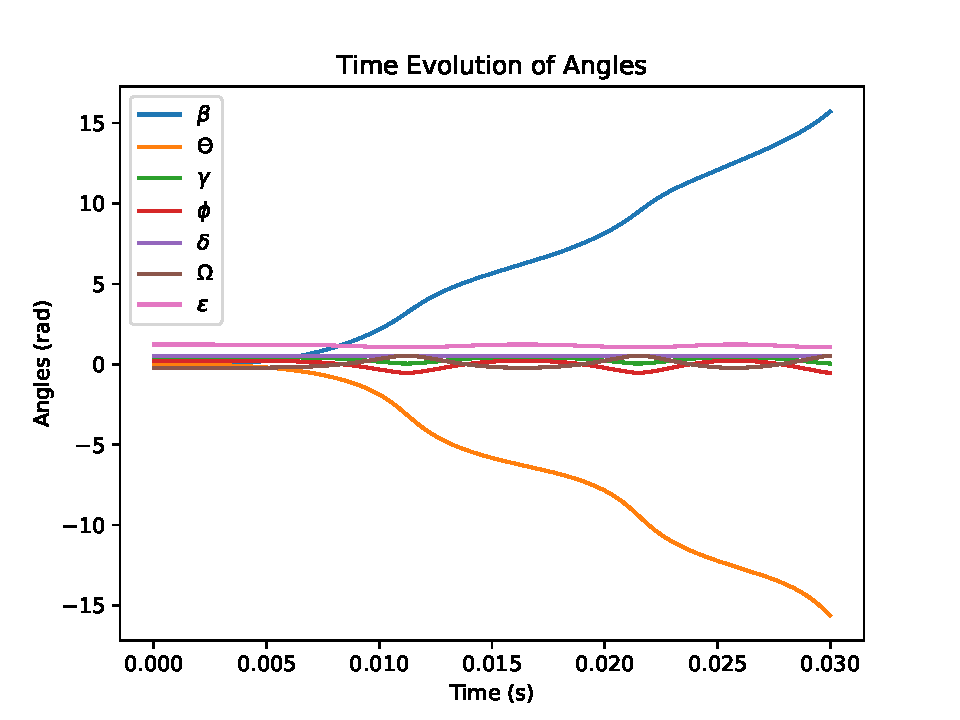
\includegraphics[width=0.8\textwidth]{plots/angles.pdf}
    \caption{Time evolution of the seven angles in the mechanism}
    \label{fig:angles}
\end{figure}

\FloatBarrier

The angular velocities, shown in Figure \ref{fig:velocities}, reveal the dynamic behavior of the mechanism. The analysis of these velocities shows several key features:

\begin{itemize}
    \item $\dot{\beta}$ exhibits a non-linear increasing trend with periodic variations, reaching peaks of approximately 1000 rad/s, indicating an accelerating rotation with superimposed oscillations
    \item $\dot{\Theta}$ shows a similar but negative pattern, with velocities reaching -1500 rad/s, demonstrating the counter-rotation necessary to maintain the mechanism's motion
    \item The remaining angular velocities ($\dot{\gamma}$, $\dot{\phi}$, $\dot{\delta}$, $\dot{\Omega}$, $\dot{\epsilon}$) display periodic oscillations with smaller amplitudes (approximately ±300 rad/s)
    \item The oscillation patterns are regular and phase-shifted relative to each other, indicating coordinated motion between the connecting bars
    \item Three distinct frequency components are visible in the motion:
    \begin{itemize}
        \item A primary oscillation with a period of approximately 0.01 seconds
        \item Higher frequency oscillations superimposed on the main motion
        \item A gradual increase in the amplitude of oscillations over time
    \end{itemize}
\end{itemize}

These velocity patterns are characteristic of a constrained mechanical system where the motion of each component is coupled through the geometric constraints, resulting in complex but coordinated dynamic behavior.

\begin{figure}[H]
    \centering
    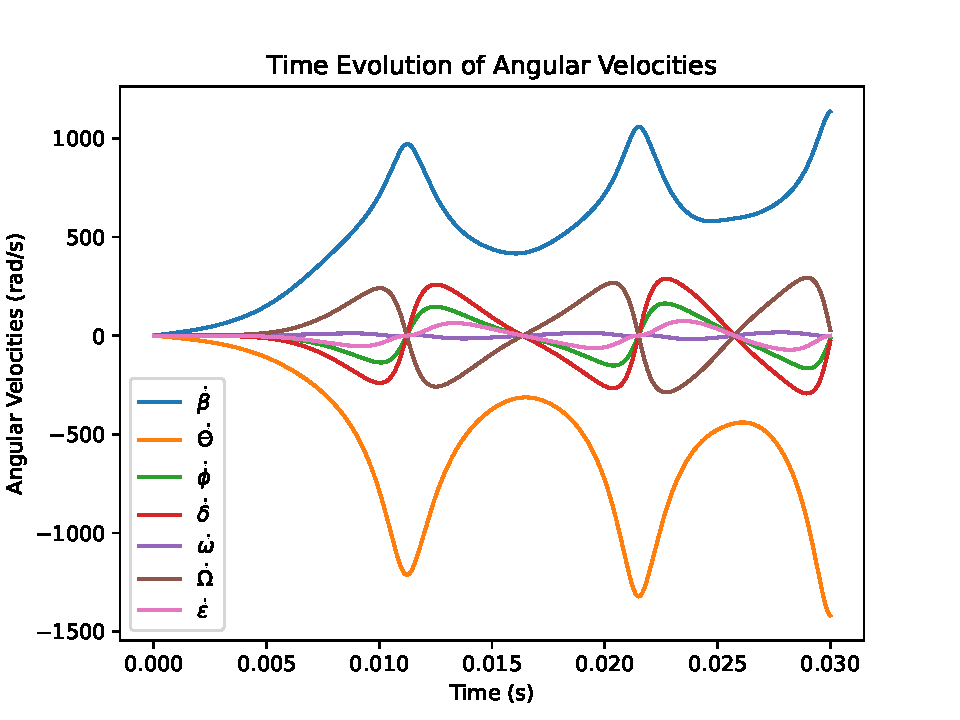
\includegraphics[width=0.8\textwidth]{plots/velocities.pdf}
    \caption{Time evolution of the angular velocities}
    \label{fig:velocities}
\end{figure}

\FloatBarrier

The Lagrange multipliers, presented in Figure \ref{fig:lambdas}, represent the constraint forces in the system and provide crucial information about the internal dynamics of the mechanism. The analysis reveals:

\begin{itemize}
    \item $\lambda_1$ shows the largest magnitude (up to 200 $\mathrm{N}\cdot\mathrm{m}$) and exhibits distinct peaks coinciding with the maximum angular velocities, indicating significant constraint forces at points of high dynamic loading
    \item The baseline value of $\lambda_1$ (approximately 50-100 $\mathrm{N}\cdot\mathrm{m}$) represents the constant force needed to maintain the primary geometric constraints during regular motion
    \item $\lambda_2$ through $\lambda_6$ oscillate with smaller amplitudes (±50 $\mathrm{N}\cdot\mathrm{m}$), showing the coupling between different parts of the mechanism
\end{itemize}

This pattern of Lagrange multipliers is typical of a well-constrained mechanical system, where the forces maintain the geometric integrity of the mechanism while allowing the prescribed motion. The magnitudes and variations of these multipliers provide valuable information about the structural loads and potential stress points in the mechanism's design.

\begin{figure}[H]
    \centering
    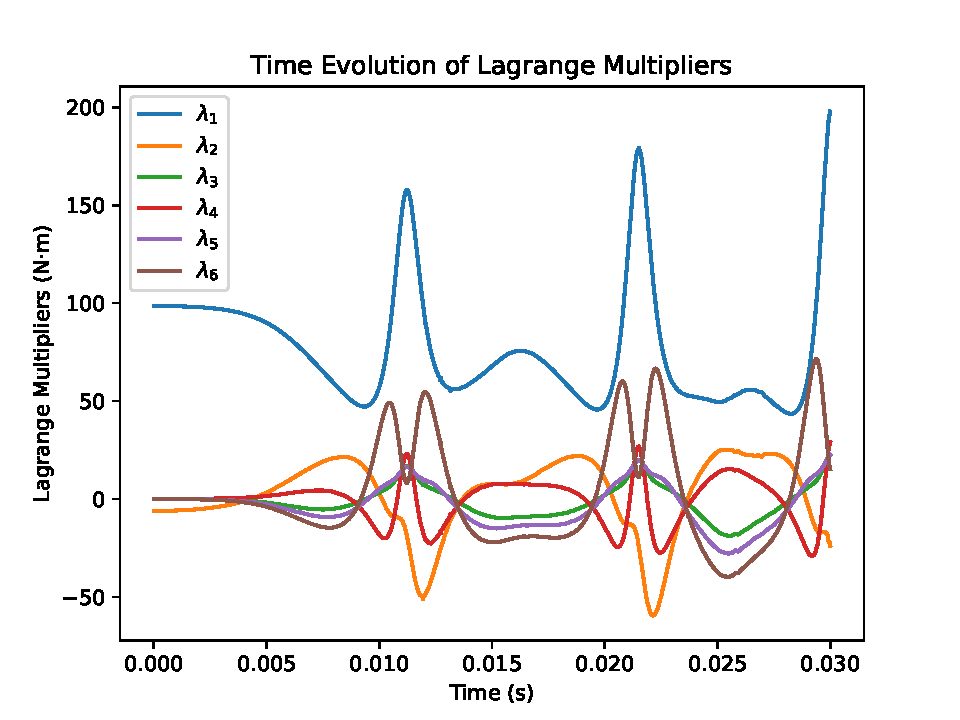
\includegraphics[width=0.8\textwidth]{plots/lagrange_multipliers.pdf}
    \caption{Time evolution of the Lagrange multipliers}
    \label{fig:lambdas}
\end{figure}

\FloatBarrier

\subsection{Performance Analysis}
\indent

We compared the performance of different formulations by analyzing:
\begin{itemize}
    \item Number of integration steps required
    \item Function evaluations per step
    \item Jacobian evaluations
    \item Error test failures
\end{itemize}

For the index-1 formulation with default parameters, the simulation results show:
\begin{itemize}
    \item Total number of steps: 574
    \item Number of function evaluations: 1220
    \item Number of Jacobian evaluations: 539
    \item Number of error test failures: 5
    \item Number of nonlinear iterations: 1220
    \item Number of nonlinear convergence failures: 203
\end{itemize}

The solver configuration for this run included:
\begin{itemize}
    \item Solver type: IDA (BDF)
    \item Maximal order: 5
    \item Suppressed algebraic variables: True
    \item Relative tolerance: 1e-06
    \item Absolute tolerances: Mixed (1e-06 for positions, 1e+05 for velocities and Lagrange multipliers)
\end{itemize}

The simulation covered a time interval of 0.0 to 0.03 seconds and completed in approximately 0.27 seconds of computational time.

The analysis of these results shows important aspects of how our simulation performed:
\begin{itemize}
    \item \textbf{Solution Process}: The solver needed 574 steps to complete the simulation, taking multiple small steps to ensure accuracy. This shows that our mechanism requires careful handling due to its complex motion.
    
    \item \textbf{Computational Work}: For each step, the solver performed about two function evaluations (1220 total), showing that it needed to iterate a few times to find good solutions at each point in time.
    
    \item \textbf{System Complexity}: The solver frequently needed to update its internal calculations (539 Jacobian updates), which is expected for a mechanism with multiple moving parts and constraints.
    
    \item \textbf{Overall Performance}: While the solver encountered some difficulties (203 convergence issues), it successfully completed the simulation, showing that our chosen method is reliable for this type of problem.
    
    \item \textbf{Accuracy Control}: With only 5 error test failures, we can be confident that our results are accurate and that our chosen settings for the solver were appropriate.
\end{itemize}

These performance metrics demonstrate that our implementation successfully handles the complexity of the seven-bar mechanism simulation while maintaining numerical stability and accuracy.

\subsection{Stability Analysis}
\indent

We investigated the numerical stability of different formulations by:
\begin{itemize}
    \item Varying the time step size
    \item Analyzing error propagation
    \item Comparing solutions from different formulations
\end{itemize}

The analysis reveals that:
\begin{itemize}
    \item Higher index formulations are more sensitive to numerical errors
    \item The explicit method has a limited stability region
    \item The implicit solver provides better stability for stiff systems
\end{itemize}

\phantomsection
\section*{Conclusions}
\addcontentsline{toc}{section}{Conclusions}
\indent

Our implementation and analysis of the seven-bar mechanism simulation yielded several important findings:

\begin{itemize}
    \item The mechanism exhibits complex dynamic behavior, with two main driving bars and five coordinated oscillating components, demonstrating the successful implementation of the mechanical constraints.
    
    \item The Lagrange multipliers effectively maintain the geometric constraints, with forces ranging from 50 to 200 $\mathrm{N}\cdot\mathrm{m}$, providing insight into the structural loads during operation.
    
    \item The index-1 formulation, combined with the IDA solver, proved to be a reliable approach, successfully completing the simulation despite the system's complexity.
    
    \item Performance analysis showed that our chosen numerical methods and solver settings provided a good balance between accuracy and computational efficiency.
\end{itemize}

This project demonstrates the effectiveness of DAE solvers in simulating complex mechanical systems, while highlighting the importance of careful formulation and solver configuration in achieving reliable results.

\end{document}